\documentclass{article}
\usepackage{spconf,amsmath,epsfig, amssymb}
\usepackage{subfigure}
\usepackage{multirow}

\def\x{{\mathbf x}}
\def\L{{\cal L}}

\title{Video Action Recognition Using Residual Vector Quantization and Hidden Markov Models}
\name{Salman Aslam, Christopher Barnes, Aaron Bobick}
\address{Georgia Institute of Technology}
\begin{document}
\maketitle


%--------------------------------------------------------------------------------------------------------------------------------------
\begin{abstract}
%--------------------------------------------------------------------------------------------------------------------------------------
In this paper, we discuss usage of a multi-stage Residual Vector Quantization (RVQ) strategy for human action recognition.  To the best of our knowledge, this is the first reported application of multi-stage RVQ to any form of video processing.  The RVQ is used to generate a single byte descriptor per image.  The evolution of these descriptors is analyzed using a bank of HMM models, one per action to be classified.  Correct classification is implemented by maximizing the posterior class conditional density.  We report comparable classification results to state of the art methods, i.e. above 90\%,  while using less than half the available training set.  
\end{abstract}

\begin{keywords}
Action recognition, residual vector quantization, $\sigma$-tree classifier, pattern recognition, machine learning, source coding, compression.
\end{keywords}


%=============================================================================================================================
\section{INTRODUCTION}
%=============================================================================================================================
Understanding human action in video is a form of high level vision processing that has received considerable interest over the past few years.  Being able to automatically detect human action can have several advantages, in areas such as surveillance, child and elderly care, crowd analysis, law enforcement and many other areas. Two basic approaches have been adopted in this regard.  The first is related to understanding human motion trajectories \cite{2001_JNL_MotionTemplates_Bobick} \cite{2007_JNL_SpaceTimeShapes_Gorelick} \cite{2010_JNL_ActionReconKinematic_Ali} while the other is related to human pose estimation \cite{2004_CNF_TrackingLooseLimbedPeople_Sigal}.  In this paper, we focus on the former approach.

Our approach is two fold.  In the first step, we use Residual Vector Quantization to represent each image in the video sequence as a single byte.  A Hidden Markov Model is then used to track the evolution of this descriptor over time.  \cite{2007_JNL_IDDM_Barnes} reports the first usage of RVQ for image analysis.  We extend that work to video analysis.  Usage of HMMs for inference in video analytics has been used by many authors~\cite{2007_CNF_HMMdynamicVideo_Hervieu}
\cite{2004_JNL_SoccerHMM_Sun}.

We first introduce some theory and notation regarding RVQ and HMMs. 
%--------------------------------------------------------------------------------------------------------------------------------------
\subsection{$\sigma$-tree Classifier and Residual Vector Quantization}
%--------------------------------------------------------------------------------------------------------------------------------------
In this paper, we use the Image Driven Data Mining approach (IDDM )introduced in \cite{2007_JNL_IDDM_Barnes}.  This approach is based on the $\sigma$-tree for data warehouse similarity searching within the pixel-block space of feature classes, and for extracting labels from knowledge base collections or "aggregates".  These collections, in this paper are foreground blobs corresponding to tracked targets.  A key difference is that the data warehouse is built on-line, and is updated every few frames as new observations of the targets under interest arrive.  Another difference is that temporal correlations are used for unsupervised learning of target labels.  To better understand the $\sigma$-tree classifier, we relate it with five well-known areas of information theory, pattern recognition and machine learning.  


First, the $\sigma$-tree classifier is a type of variable rate vector quantizer \cite{2003_JNL_HighRateVQDetection_Hero}.  Second, Truncel \emph{et al} explore the relationship between rate-distortion theory and content-based retrieval in high dimensional databases \cite{2004_JNL_RateDistortionVsDatabases_Truncel}.  Third, the $\sigma$-tree design problem parallels the joint codebook design problem addressed in the source coding literature for multiple stage vector quantization \cite{1996_JNL_AdvancesRVQ_Barnes}.  Fourth, the $\sigma$-tree classifier can be compared to dimensionality reduction methods such as Principal Components Analysis (PCA).  PCA seeks to reorient the basis vectors in $\mathbb{R}^k$ and achieves compression by ignoring projected data components with least variances.  Even though a $\sigma$-tree classifier can be used to achieve lower dimensionality, it primarily seeks to partition $\mathbb{R}^k$ like other well known classifiers such as neural networks and support vector machines \cite{2007_JNL_IDDM_Barnes}.  Further, note that neural networks partition the decision space with hyperplanes or hypersurfaces, depending on whether or not hidden layers are used.  Support vector machines also do partition the decision space, but with hyperplanes in a higher dimension space that separate the data with maximum margin.  The $\sigma$-tree classifier tesselates the decision space $\mathbb{R}^k$ with $k$ Voronoi cells, the geometric dual of delaunay triangulation in $\mathbb{R}^2$.  The fifth and final comparison is with the well-known $k$-means algorithm, or the Linde Buzo Gray (LBG) algorithm as it is more commonly referred to in the source coding literature.  It is also called the Generalize Lloyd Algorithm (GLA).  Most vector quantization methods use this algorithm to create cluster centroids \cite{1991_BOOK_VQ_GershoGray}.  Indeed, the $\sigma$-tree classifier centroids can also be designed using this algorithm.  For a concrete and simple example of a $\sigma$-tree, see \cite{2007_JNL_IDDM_Barnes}.


The mechanism that allows a $\sigma$-tree to be built is multi-stage Vector Quantization (VQ), also called Residual Vector Quantization (RVQ) or Direct Sum Successive Approximation (DSSA) Vector Quantization.  These three terms will be used interchangeably in this paper.  Juang and Gray first proposed the RVQ structure \cite{1982_CNF_SpeechRVQ_JuangGray} and suggested that RVQ stages be designed by sequential application of GLA.  The main shortcoming of this approach is that each stage codebook is generated while considering only the error due to the previous stages (the \emph{causal error}); the error due to subsequent stages (the \emph{anticausal error}) is ignored.  A joint design approach on the other hand takes into account both the causal and anticausal errors to reduce the \emph{total error}.  Various techniques have been proposed for joint optimization.  We now introduce notation and define "joint optimality."

The $pth$ stage of a $P$-stage RVQ, with $N$ codevectors per stage, is a $k$-dimensional VQ defined by the mapping 
\begin{equation}
Q_p : \mathbb{R}^k \mapsto C_p
\end{equation}
  
Here, $\mathbb{R}^k$ is the $k$-dimensional input space,   

\begin{equation}
C_p = \{y_p(0), y_p(1), \ldots y_p(N_p - 1) \}
\end{equation}

is the $pth$-stage codebook and $y_p(i_p) \in \mathbb{R}^k$ is a $pth$-stage \emph{codevector}.  
Residual quantizer stage mappings $Q_p$ are collectively equivalent to a single mapping,

\begin{equation}
Q : \mathbb{R}^k \mapsto C
\end{equation}



Here, $C$ is the \emph{direct sum codebook} and is the direct sum of the stage codebooks $C=C_1 + C_2 + \ldots C_p$.  
In practice, the stage mappings $Q_p(.)$ are realized as a composition of a stage encoder mapping $E_p = \mathbb{R}^k \mapsto I_p$, and a stage decoder mapping $D_p: I_p \mapsto C_p$, that is $Q_p(x_1) = D_p[E_p(x_1)]$, where $x_1$ is a realization of $X_1$, which is the random source output.  


%The direct sum codebook is the direct sum of the stage codebooks $C=C_1 + C_2 + \ldots C_p$.  In practice, the stage mappings $Q_p$ %are realized as a composition of a stage encoder mapping $E_p: $
An RVQ is said to be jointly optimal if a local or global minimum value of the average distortion $d(E,D) = E[m(X_1, D(E(X_1)))]$ is achieved, where $m(.,.)$ is a distortion metric, and E[.] is the expectation operator.  This shows that an RVQ is a product code VQ with a direct sum codebook structure \cite{1993_JNL_RVQDSC_Barnes}.  Also notice that computation (search) and memory (storage) requirements are proportional to $kNP$.  So, the cost functional grows linearly with classifier dimensionality $k$, branch multiplicity $N$, and the number of tree levels $P$.  However, the number of indexing options is $N^P$.  This computational advantage makes it possible to use RVQ in real time tracking, even though the data dimensionality is very high.

%A near neighbor search is proportional in computational complexity to $MP$ whereas there is one of $M^P$ possible outcomes.
%Different types of VQ deal with how the partitions are created, indexed, or searched.  An RVQ is different from a traditional VQ in the sense that it partitions $\mathbb{R}^k$ into $M$ cells.  The residual space, also in $\mathbb{R}^k$, is then partitioned again into $M$ cells.  This process is repeated $P$ times.  The advantage of this approach is that in obtaining $M^P$ partitions, we need to run our partitioning algorithm $P$ times and generate $M$ partitions at each stage.  In traditional VQ, the partitioning algorithm would run once but have to create $M^P$ partitions.  For the binary case, i.e. two templates per stage, $M=P$, and if 8 stages are used, we require only 16 searches, whereas in traditional VQ, this would require 256.  

%%--------------------------------------------------------------------------------------------------------------------------------------
%\subsection{Background Subtraction}
%%--------------------------------------------------------------------------------------------------------------------------------------
%Several preprocessing steps may be required before tracking can be initiated.  These could include image stabilization, normalization, and downsampling.  The final preprocessing step in most cases is background modeling.  Several algorithms have been developed for this task.  Most of these algorithms depend on appearance modeling.  A detailed overview alongwith a graphical comparison of how these algorithms perform on the canonical problems in foreground detection is given in \cite{1999_CNF_Wallflower_Toyama}.  In this paper, we use the Multi Gaussian algorithm~\cite{2000_JNL_MG_Stauffer}.  In this algorithm, the grayscale value of each pixel is tracked over time and represented as a mixture of $K$ Gaussian distributions.  The mean and variance of the Gaussians is tracked over time.  This is a pixel based approach with no region based processing.  However a post processing step of morphological operations, connectedness constraints, and area thresholding makes the combined approach quite robust to slow drifts in appearances.  The probability of observing the current pixel value at time, $x_t$, is 
%
%\begin{equation}
%p(x_t)=\sum_{i=1}^{K}\omega_{i,t}*\eta(X_t, \mu_{i,t}, \Sigma_{i,t})
%\end{equation}
%
%where $K$ is the number of distributions,  $\omega_{i,t}$ is an estimate of the weight of the $i$th Gaussian in the mixture at time $t$.  The gaussian distributions are given by,
%
%\begin{equation}
%\eta(x_t, \mu, \Sigma)=\frac{1}{(2\pi)^\frac{n}{2}|\Sigma|}e^{-\frac{1}{2}(X_t-\mu_t)^T\Sigma^{-1}(X_t-\mu_t)}
%\end{equation}
%
%  The pixel process is not stationary, and so one cannot resort to maximizing the likelihood of the observed data using the Expectation Maximization (EM) algorithm.  Instead, the weights of the Gaussians are adjusted as follows,
%
%\begin{equation}
%\omega_{k,t} = (1-\alpha) \omega_{k,t-1} + \alpha M_{k,t}
%\end{equation}
%
%where $\alpha$ is the learning rate, and $M_{k,t}$ is 1 for the model which matched and 0 otherwise.  A match is defined as a pixel within 2.5 standard deviations of a distribution.  In this paper, we use a value of $K=3$. 

%%--------------------------------------------------------------------------------------------------------------------------------------
%\subsection{Tracking}
%%--------------------------------------------------------------------------------------------------------------------------------------
%Multi-target tracking is a complex, but well studied problem.  \cite{2006_JNL_TrackingSurvey_MubarakShah} provides a comprehensive overview of this area.  
%The problem can be further compounded if a perspective projection is used.  During initialization, every observation can be assigned a target.  In the absence of velocity information, a state estimation algorithm such as the Kalman or Particle Filter cannot be initialized.  Maintaining multiple hypotheses In subsequent frames, To reduce the combinatorial possibilities of target location in the subsequent frames during this training period, the number of possible directions can be quantized to a limited number of levels.    Therefore, in order to reduce the complexity of the comThe number of possible directions that the target can move in can be quantized to reduce the possibilities of where the targets could be in the next frame.  In the absence of velocity information,   Tracks are initialized at frame 0.  In the 2D tracking case in which 

%%--------------------------------------------------------------------------------------------------------------------------------------
%\section{Particle Filter}
%%--------------------------------------------------------------------------------------------------------------------------------------
%The particle filter is a powerful tool in Bayesian estimation if the system is non-linear and/or the noise is non-Gaussian.  In such cases, the (Extended) Kalman Filter may exhibit poor performance [11].  In this case, one is forced to look beyond the Kalman filter.  The particle filter is a popular mechanism employed in such cases although its main disadvantage is its computational load.  
%Consider the standard filtering formulation
%Here, xk   Rn is the state vector of the system, a, b: RnxR Rn and c: RnxR Rm are vector valued functions.  wk is the process noise, vk is the measurement noise, and they are both white sequences with known distribution. po(x) is a known distribution for the initial state xo.  Furthermore, it is assumed that wk, vk and xo are independent.  Zk := {z1, z2, � } is the observation vector.  Then, when an observation arrives, i.e. a realization of Zk, the filtering problem is to find the best estimate of x given Zk.  In the linear Gaussian case, p(xk|Zk) is also Gaussian and the Kalman filter provides an optimal closed form solution.  In the non-linear and/or non-Gaussian case, the Kalman filter may not provide an adequate solution.  Using Bayes' Rule, it is known that,
%
%            (5)
%The Kalman filter is a closed form solution for the above equation for the linear Gaussian case.  An approximate solution is the so called sampling filter approach.  The core of the sampling filter algorithm is that the above equation is approximated on the basis of an N point grid in the state space [12].  
%
%The basic idea behind the particle filter is that we represent the posterior distribution of interest with a set of weighted particles, each of which forms an independent hypothesis of the state at a given time [13].  The weights have to be chosen correctly for this weighted set of particles to be representative of the posterior distribution.  To get an estimate of the state, MAP or MMSE estimates can be used, although in our experience, the MAP estimate tends to work better.  In the first step, a set of particles from the previous time step are used to propose a new setup for the new time step.  In the second step, these are weighted to ensure consistency.  Finally, the weighted particles are resampled to convert them into an unweighted set without changing the distribution they represent.  
			\begin{figure}				
					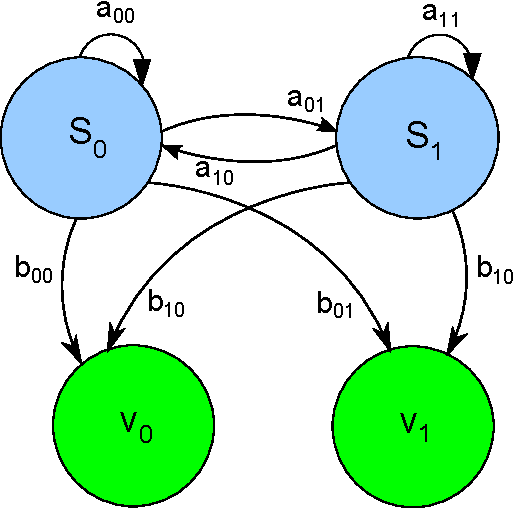
\includegraphics[width=.30\textwidth]{figs/RVQ_HMM_IPCV2010_HMMblockDiagram}
					\centering
					\caption{Hidden Markov Model.}
					\label{fig:HMM}
			\end{figure}
			
\subsection{Hidden Markov Model}
%-------------------------------
A comprehensive overview of HMMs can be found in \cite{1989_JNL_TutorialHMM_Rabiner}.  The goal is to analyze a sequence of random variables.  We relax the constraint of independence at the cost of sacrificing the factorization of the joint distribution going from a product of marginal distributions to a product of conditional distributions.  An HMM (Figure~\ref{fig:HMM})is characterized by the following:  

					\begin{figure}				
					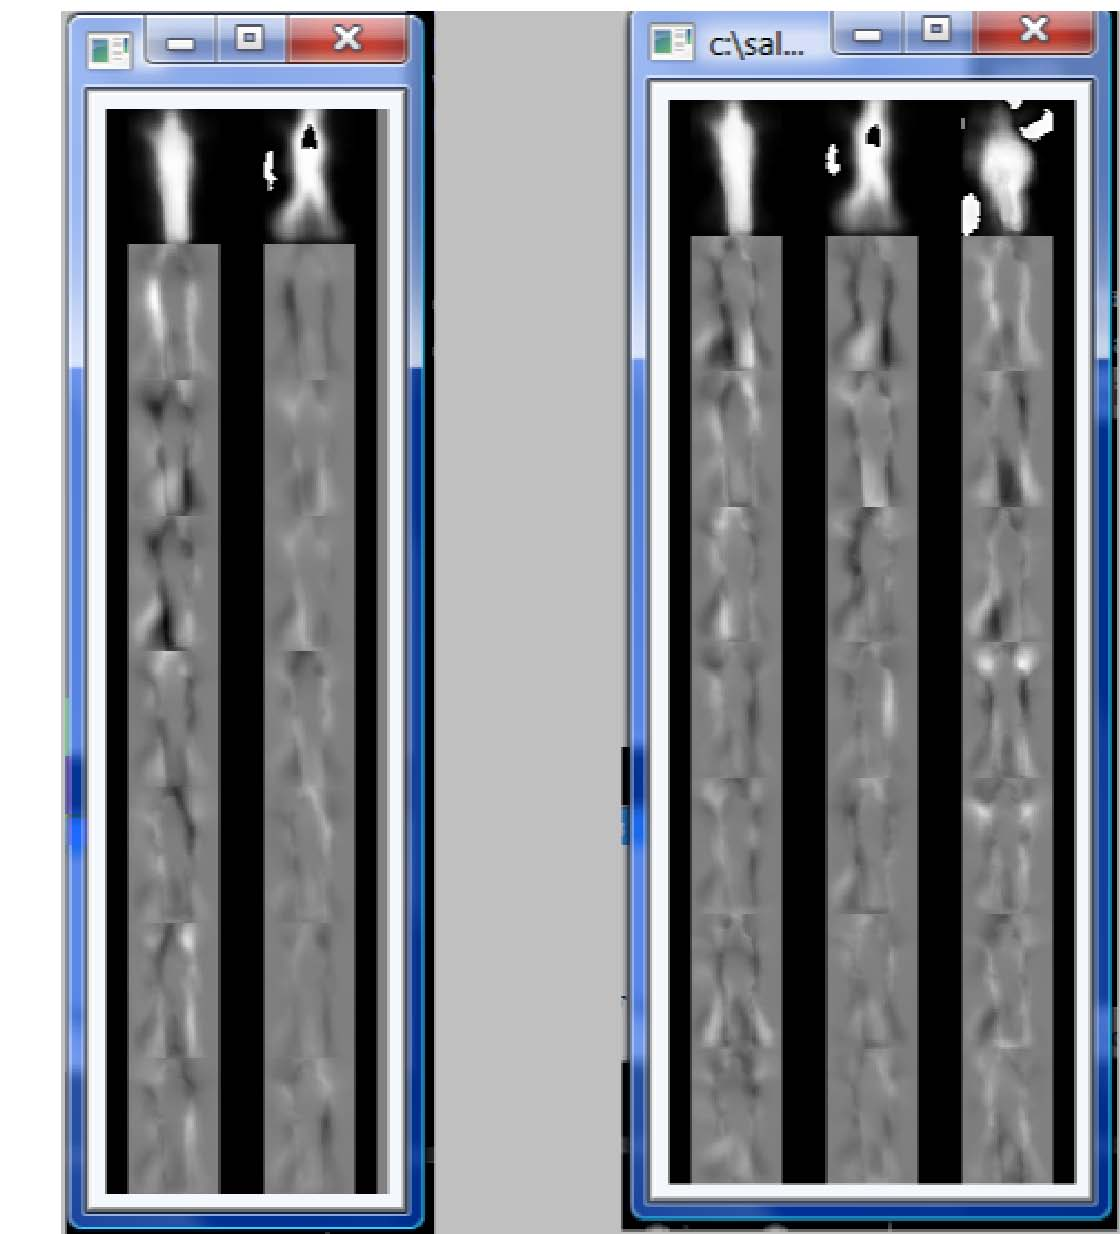
\includegraphics[width=.50\textwidth]{figs/RVQ_HMM_IPCV2010_codebooks}
					\centering
					\caption{RVQ codebooks.  With 2 templates per stage, and 8 stages, a total of 256 leaf nodes are possible.  With 3 templates per stage, a total of 6561 leaf nodes are possible.}
					\label{fig:codebooks}
			\end{figure}	


					\begin{figure}	
					\centering			
					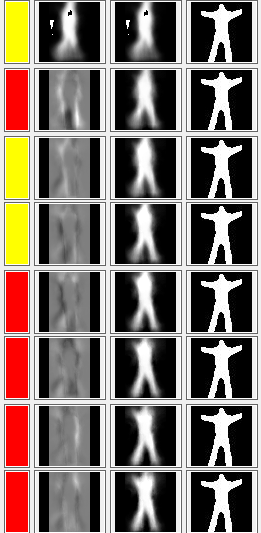
\includegraphics[width=.25\textwidth]{figs/RVQ_HMM_IPCV2010_reconstruction_jack___moshe__00022___79x109}
					\caption{Image reconstruction using direct sum successive approximation RVQ.}
					\label{fig:reconstruction}
			\end{figure}	
			
								\begin{figure}				
					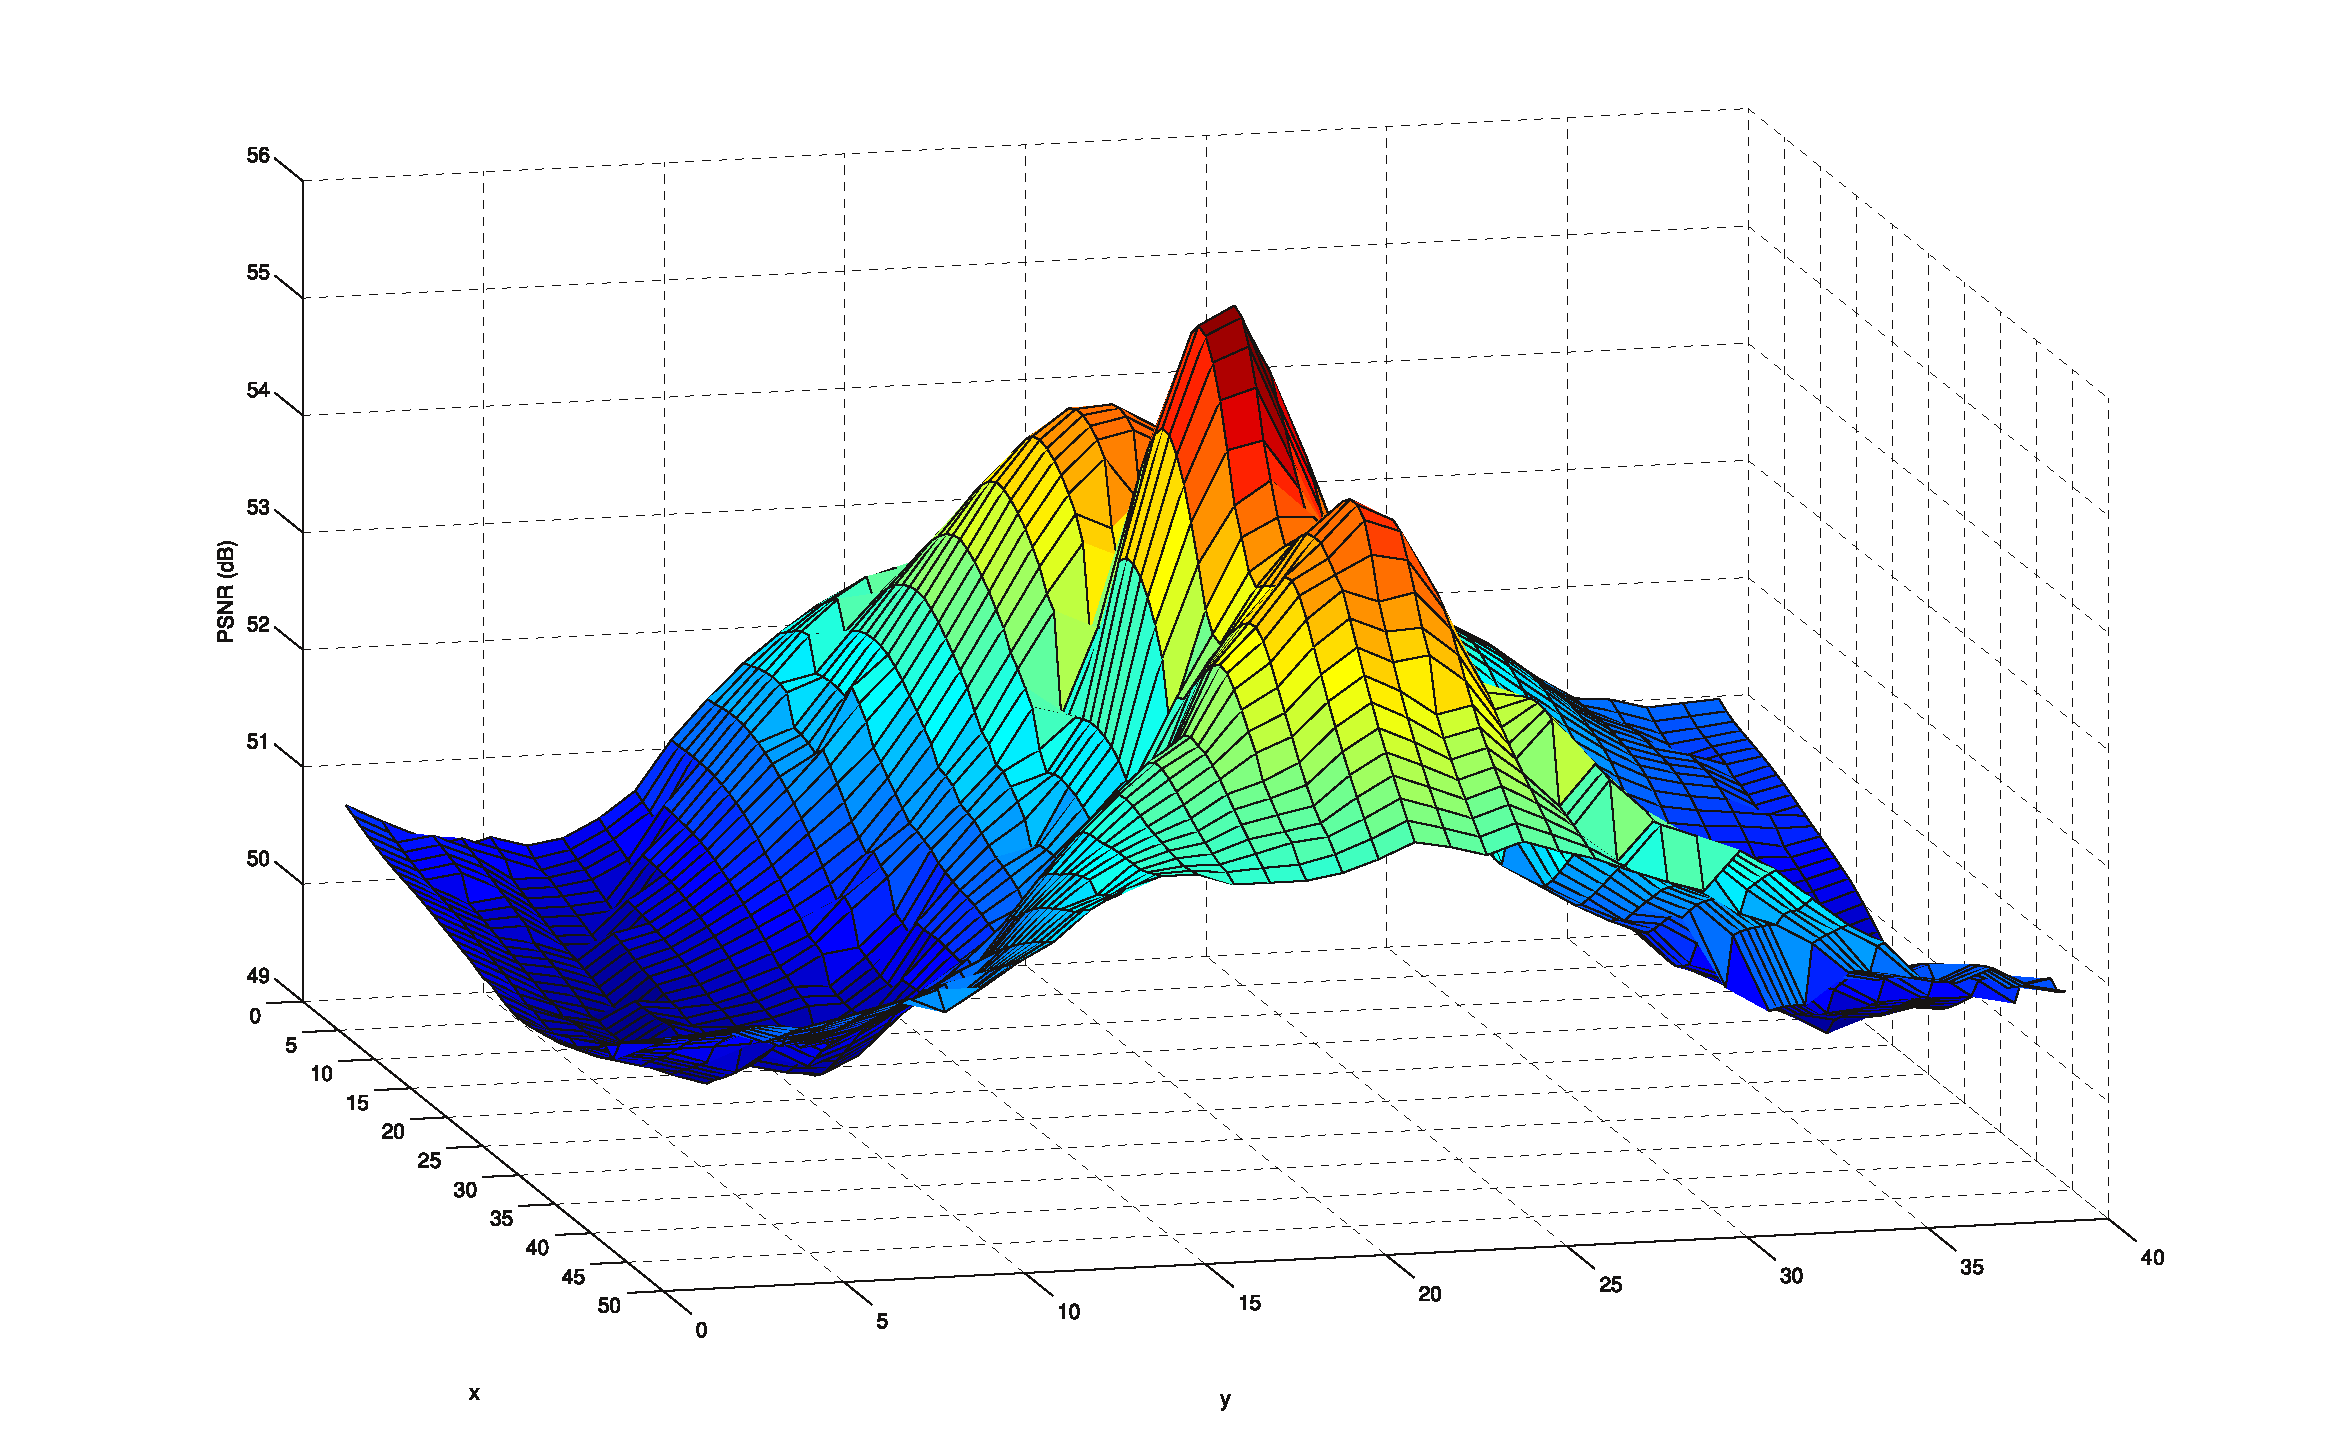
\includegraphics[width=.50\textwidth]{figs/RVQ_HMM_IPCV2010_reconstructionPSNRfromCORfile_jack___moshe__00022___79x109}
					\centering
					\caption{PSNR values of reconstruction computed at every point of the test image.}
					\label{fig:corFile}
			\end{figure}
			
								\begin{figure*}		
								\centering		
					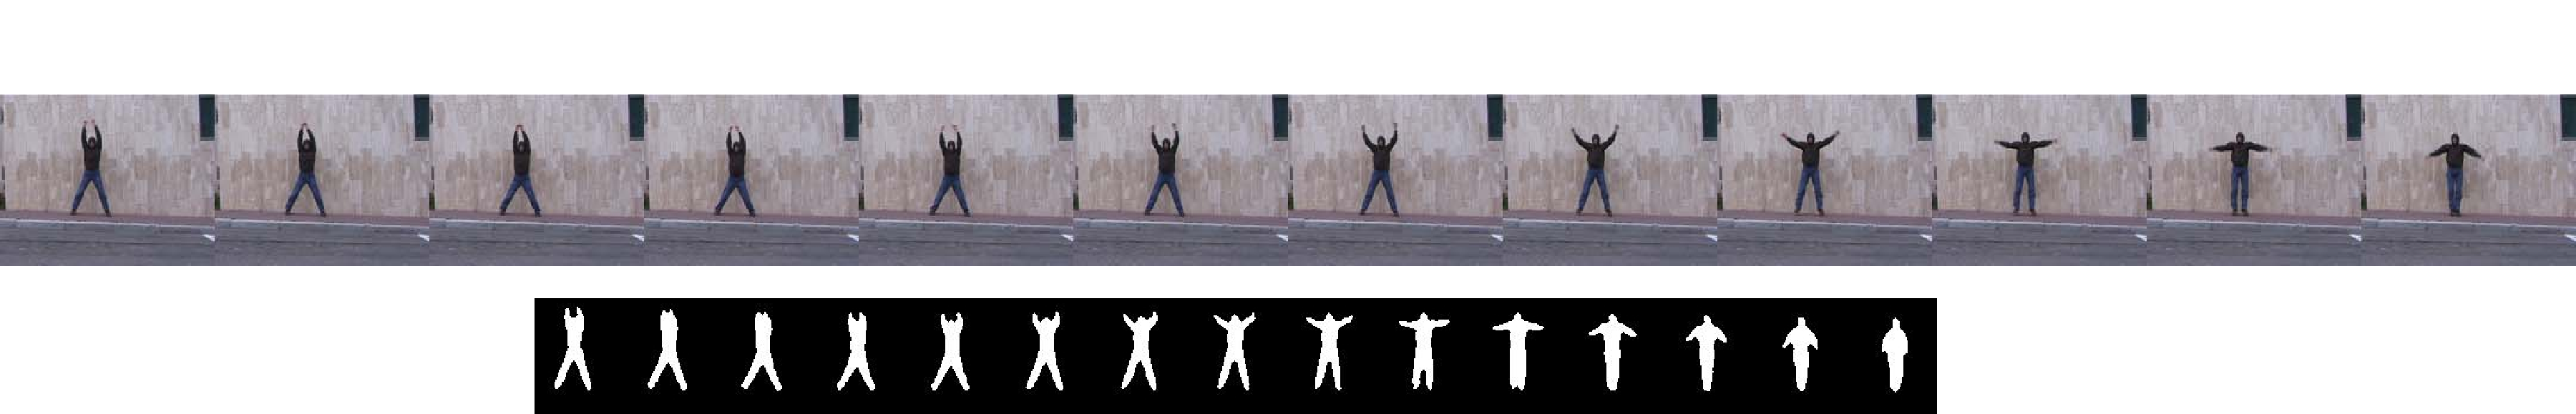
\includegraphics[width=1.0\textwidth]{figs/RVQ_HMM_IPCV2010_WeizmannSequenceSnapshot}
					\centering
					\caption{Sample images from the Weizmann dataset.}
					\label{fig:sequence}
			\end{figure*}
			
						
\begin{enumerate}
\item \textbf{Number of states in the model, N}: We denote the individual states as $S={S_1, S_2, ... S_N}$ and the state at time $t$ as $q_t$.
\item \textbf{Number of distinct observation symbols per state, M}: This is the discrete alphabet size.    We denote the individual symbols as $V={v_1, v_2, ... v_M}$.
\item \textbf{State transition probability distribution}.  For the special case where every state can reach every other state, $a_ij>0$.
\begin{equation}
a_{ij} = p(q_{t+1}=S_j|q_t=S_i)  \ \ \ \ \ 1 \leq i, j \leq N
\end{equation}
\item \textbf{Observation symbol probability distribution}. 
\begin{equation}
b_{jk} = p(v_k|q_t=S_j)  \ \ \ \ \ 1 \leq j \leq N,  1 \leq k \leq M
\end{equation}
\item \textbf{Initial distribution}.
\begin{equation}
\pi_i	= P(q_1=S_i) \ \ \ \ \ 1 \leq i \leq N
\end{equation}
\end{enumerate}

An HMM, defined by $N, M, A, B, \pi$, can be used to generate a sequence of observation symbols, $O_1, O_2, ... 	O_T$, and as a model for how a given observation was generated by an appropriate HMM.  For convenience, we use
\begin{equation}
\lambda = (A, B, \pi)
\end{equation}
to indicate the complete parameter set of the model.  Each observation $O_t$ is one of the symbols from $V$ and $T$ is the number of observations in the sequence.  

In HMMs, there are 3 basic problems: (a) Given an observation sequence, what is the probability of a particular model generating that sequence.  This is solved efficiently using the Forward Backward Algorithm. (b) Training the model.  This is done using the EM Algorithm.  (c) Finding the most likely sequence of state evolution.  This is solved using the Viterbi algorithm.  In our case, we are interested in the first application, i.e. given a sequence of observing human actions, what is the most probable label for that action.  Mathematically, what is the likelihood of observing the given sequence,
%
%\begin{itemize}
%\item \textbf{Testing}.  Given the observation sequence $O_1, O_2, ... O_T$, and a model $\lambda=(A, B, \pi)$, how do we compute
%\begin{itemize}
%\item $p(O|\lambda)$ (Evaluation problem.)  Use of forward backward algorithm.
%\item  Use Viterbi algorithm
%\begin{equation} 
%\max_{q_1, q_2, ... q_T}p(q_1, q_2, ... q_t, O_1, O_2, ... O_t|\lambda)
%\end{equation}
%\end{itemize}
%\item \textbf{Training}.  How do we adjust the model parameters $\lambda=(A, B, \pi)$ to maximize $p(O|\lambda)$.  Use Baum Welch algorithm.
%\end{itemize}
%
%\subsubsection{Problem 1}
%%------------------------

\begin{align}
	\label{eq:HMM_problem1_evaluation_ie_likelihood1}
	p(\textbf{O}_n| \textbf{Q}_n) 
	&= \frac{p(\textbf{O}_n, \textbf{Q}_n)				}   	{p(\textbf{Q}_n)}  	\notag	\\
%	&= \frac{p(o_n, \textbf{O}_{n-1}, \textbf{Q}_n)					  }   	{p(\textbf{Q}_n)}  	\notag	\\
%	&= \frac{p(o_n| \textbf{O}_{n-1}, \textbf{Q}_n)					  p(\textbf{O}_{n-1}, \textbf{Q}_n)}   	{p(\textbf{Q}_n)}  	\notag	\\
%	&= \frac{p(o_n| q_n)                           				p(\textbf{O}_{n-1}, \textbf{Q}_n)}   	{p(\textbf{Q}_n)}		\notag	\\  
%	&= \frac{p(o_n| q_n) p(o_{n-1}|\textbf{O}_{n-2}, \textbf{Q}_n) p(\textbf{O}_{n-2}, \textbf{Q}_n)}   	{p(\textbf{Q}_n)}	\notag	\\ 
%	&= \frac{p(o_n| q_n)p(o_{n-1}|q_{n-1}) p(\textbf{O}_{n-2}, \textbf{Q}_n)}   	{p(\textbf{Q}_n)}		\\  	
%	&= \frac{p(o_n| q_n)p(o_{n-1}|q_{n-1}) ... p(o_{2}|q_{2})p(o_1|q_1) p(\textbf{Q}_n)}   	{p(\textbf{Q}_n)}		\notag	\\  	
	&= p(o_n| q_n)p(o_{n-1}|q_{n-1}) ... p(o_2|q_2)p(o_1|q_1)		  	
\end{align}








%For the prior distribution,
%\begin{align}
%	\label{eq:HMM_prior}
%		p(\textbf{X}_n) 
%	&= p(x_n| \textbf{X}_{n-1})p(\textbf{X}_{n-1})   	  	\notag	\\
%	&= p(x_n| x_{n-1}) p(\textbf{X}_{n-1})   			\\  
%	&= p(x_n| x_{n-1}) p(x_{n-1}| \textbf{X}_{n-2})p(\textbf{X}_{n-2})  \notag \\	
%	&= p(x_n| x_{n-1}) p(x_{n-1}| x_{n-2}) ... p(x_2|x_1)p(x_1)  \notag	
%\end{align}
%
%For the likelihood distribution,
%\begin{align}
%	\label{eq:HMM_problem1_evaluation_ie_likelihood}
%	p(\textbf{Z}_n| \textbf{X}_n) 
%	&= \frac{p(\textbf{Z}_n, \textbf{X}_n)				}   	{p(\textbf{X}_n)}  	\notag	\\
%	&= \frac{p(z_n, \textbf{Z}_{n-1}, \textbf{X}_n)					  }   	{p(\textbf{X}_n)}  	\notag	\\
%	&= \frac{p(z_n| \textbf{Z}_{n-1}, \textbf{X}_n)					  p(\textbf{Z}_{n-1}, \textbf{X}_n)}   	{p(\textbf{X}_n)}  	\notag	\\
%	&= \frac{p(z_n| x_n)                           				p(\textbf{Z}_{n-1}, \textbf{X}_n)}   	{p(\textbf{X}_n)}		\notag	\\  
%	&= \frac{p(z_n| x_n) p(z_{n-1}|\textbf{Z}_{n-2}, \textbf{X}_n) p(\textbf{Z}_{n-2}, \textbf{X}_n)}   	{p(\textbf{X}_n)}	\notag	\\ 
%	&= \frac{p(z_n| x_n)p(z_{n-1}|x_{n-1}) p(\textbf{Z}_{n-2}, \textbf{X}_n)}   	{p(\textbf{X}_n)}		\\  	
%	&= \frac{p(z_n| x_n)p(z_{n-1}|x_{n-1}) ... p(z_{2}|x_{2})p(z_1|x_1) p(\textbf{X}_n)}   	{p(\textbf{X}_n)}		\notag	\\  	
%	&= p(z_n| x_n)p(z_{n-1}|x_{n-1}) ... p(z_2|x_2)p(z_1|x_1)		\notag  	
%\end{align}

%For the posterior distribution,
%\begin{align}
%	\label{eq:HMM_posterior}
%	p(\textbf{X}_n| \textbf{Z}_n) &= \sum_\textbf{X} p(\textbf{Z}_n| \textbf{X}_n) p(\textbf{X}_n) 
%\end{align}	
%\subsection{Forward Backward Algorithm}


%--------------------------------------------------------------------------------------------------------------------------------------
\section{EXPERIMENTS}
%--------------------------------------------------------------------------------------------------------------------------------------
Our approach, as mentioned earlier is two fold.  The first step is generating a descriptor for every image using RVQ.  The second step involves tracking the evolution of this descriptor using an HMM.  We use the Weizmann database (Figure~\ref{fig:sequence}) reported in \cite{2007_JNL_SpaceTimeShapes_Gorelick} and compare our results with other researchers who have used this database as well for similar purposes~\cite{2007_JNL_SpaceTimeShapes_Gorelick} \cite{2001_CNF_EventBasedAnalysisVideo_Manor} 
\cite{2010_JNL_ActionReconKinematic_Ali}.  \cite{2007_JNL_SpaceTimeShapes_Gorelick} uses the solution to the Poisson equation to extract a wide variety of useful local shape properties.  \cite{2001_CNF_EventBasedAnalysisVideo_Manor} proposes a statistical measure between video sequences based on their behavioral content.  \cite{2010_JNL_ActionReconKinematic_Ali} uses kinematic features of optical flow of human motion to understand human action.   

We separate the dataset into training and test images.  An RVQ codebook is generated using the training dataset (Figure~\ref{fig:codebooks}).  This one time offline step takes approximately 6 minutes on a Core2 Duo 2.5 GHz laptop for a total of 2400 images.  An image reconstruction using direct sum successive approximation with this codebook is shown in Figure~\ref{fig:reconstruction}.  Generating descriptors for the images takes another 3 minutes, and this is also an offline step.  This time includes GUI related instructions as well as accessing an SQL Server database.  These steps are accomplished using the C language.  Figure~\ref{fig:corFile} shows the PSNR value of image reconstruction for every point inside the image.  Notice that the highest PSNR is at the center, essentially showing that this is the centroid of the human at that point in the sequence.  Training an HMM takes around 700 msec in Matlab.  The online task of computing the class conditional probabilities takes 1.1 msec per frame in Matlab.   

We are trying to identify 10 actions, walk (a1), run (a2), skip (a3), jumping jacks (a4), jumping (a5), in place jumping (a6), sideways motion (a7), waving with one hand (a8), waving with two hands (a9) and bending (a10).  There are a total of 8 users.  To test the actions of particular user, we train our system on all the other users.  This process is repeated for all users one at a time.

			\begin{figure*}				
					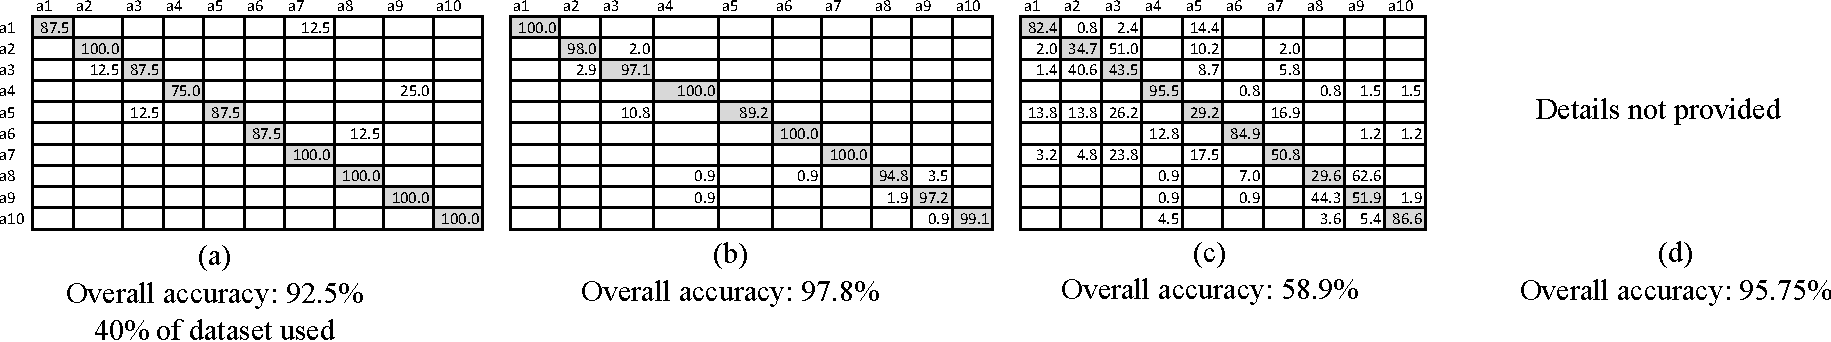
\includegraphics[width=1.0\textwidth]{figs/RVQ_HMM_IPCV2010_tabularResults}
					\centering
					\caption{Action confusion matrix.  We compare classification performance of our approach on 10 actions, walk (a1), run (a2), skip (a3), jumping jacks (a4), jumping (a5), in place jumping (a6), sideways motion (a7), waving with one hand (a8), waving with two hands (a9) and bending (a10) with other researchers using the same Weizmann dataset. (a) Our method, produces accurate results despite using less than half the training data. (b) Method reported in \cite{2007_JNL_SpaceTimeShapes_Gorelick}. (c) Method reported in \cite{2001_CNF_EventBasedAnalysisVideo_Manor} (d) Method reported in \cite{2010_JNL_ActionReconKinematic_Ali}.}
					\label{fig:Table}
			\end{figure*}




%--------------------------------------------------------------------------------------------------------------------------------------
\section{RESULTS}
%--------------------------------------------------------------------------------------------------------------------------------------
Our results, and a comparison with other researchers is given in Table~\ref{fig:Table}.  It is worth mentioning that we use around 40\% of the images for training.  Since the dataset is based on 50 fps video, this is about half a second of training video per action.  Yet, Table~\ref{fig:Table} shows that our classification accuracy is comparable with other methods that use the entire database.  Notice that the greatest error is in classifying jumping jacks as waving with two hands, since these two actions are very similar.  Moreover, since we use very few images, this is understandable.  


%--------------------------------------------------------------------------------------------------------------------------------------
\section{CONCLUSIONS}
%--------------------------------------------------------------------------------------------------------------------------------------
We demonstrate the first reported application of multi-stage residual vector quantization to any form of video processing.  In this paper, the application we focus on is human action recognition using HMMs as an inference engine over an RVQ generated sequence of image descriptors.  We demonstrate comparable performance with other state of the art methods, but using less than half the number of training images.  Our future work will focus on temporal evolution of the codebooks for time adaptive analysis of human motion evolution.

%--------------------------------------------------------------------------------------------------------------------------------------
%BIBLIOGRAPHY
%--------------------------------------------------------------------------------------------------------------------------------------
\bibliographystyle{IEEE}
\bibliography{MyCitations}
\end{document}
